\documentclass[a4paper, 12pt, twoside, openright]{mythesis}

\renewcommand{\baselinestretch}{1}       % for squeezing the draft into the page limit, do not use

% Note
% Use \textsc{Name} to separate images, videos, dataset names from the main texts.

% =============================================================================
% Commonly used packages
% =============================================================================

% For removing Package ifpdf Error
%%%%%%\let\ifpdf\relax

% For removing LaTeX Font Warning
\usepackage{lmodern}

% Add Reference in Contents
\usepackage[nottoc]{tocbibind}

% Figures
%\usepackage{subcaption}
\usepackage{float}
%\usepackage[justification=raggedright]{caption}	% makes captions ragged right - thanks to Bryce Lobdell
\usepackage{lscape} % Useful for wide tables or figures.
\usepackage{makecell}
\usepackage{sidecap}

\graphicspath{{figures}{example}}

% Algorithm
\usepackage[lined,ruled,linesnumbered]{algorithm2e}
\usepackage{algorithmic}

% Table and list
\usepackage{booktabs} % Publication quality tables
\usepackage{multirow}
\usepackage{rotating} % sideways
\newcommand{\vergap}[1]{\renewcommand{\arraystretch}{#1}}
\newcommand{\horgap}[1]{\setlength{\tabcolsep}{#1}}
%\specialrule{width}{abovespace}{belowspace}
\newcommand{\dtoprule}{\specialrule{2pt}{0pt}{2pt}}
\newcommand{\dbottomrule}{\specialrule{2pt}{0pt}{\belowrulesep}}

\usepackage{paralist}
\usepackage{enumitem}

% Math
\usepackage{bm} % Make bold, italic math symbols
\usepackage{epsfig} % for figures
\usepackage{graphicx} % another package that works for figures
\usepackage{times}
%\usepackage{mathptmx}
\usepackage{mathtools}
\usepackage{textcomp, gensymb} % math symbol
\usepackage{amssymb,amsmath,amsfonts} % Short math guide for LaTeX ftp://ftp.ams.org/pub/tex/doc/amsmath/short-math-guide.pdf
\usepackage{siunitx} % SI units
\newcommand{\norm}[1]{\left\lVert#1\right\rVert}
\newcommand{\cp}[1]{\left[#1\right]_{\times}}

% Fonts
\usepackage{units}
\usepackage{color}

% Comments
\usepackage{comment}

% Hyperlinks
\usepackage{url} % Hyphenation of URLs.
\usepackage{xcolor}
\usepackage[backref=page]{hyperref}
\hypersetup{colorlinks,breaklinks,
            urlcolor=[rgb]{0.918,0,0.545},
            linkcolor=[rgb]{0.710,0.180,0.141},
            citecolor=[rgb]{0,0.545,0.447}}
\usepackage{bookmark}
%\usepackage[pagebackref=true,breaklinks=true,colorlinks,bookmarks=false]{hyperref} % remove letterpaper=true,
%
%\usepackage{slashbox}
\usepackage[table,caption=false]{xcolor}
%\usepackage{setspace}

% Better hyphenation
\usepackage{microtype}

% Appendix
\usepackage[toc,page]{appendix}

% =========================================
% Useful macros
% =========================================

% Latin abbreviations
\newcommand{\etal}{\textit{et al}.~} % ``and others'', ``and co-workers''
\newcommand{\eg}{e.g.,~} % ``for example''
\newcommand{\ie}{i.e.,~} % ``that is'', ``in other words''
\newcommand{\suchthat}{\, \mid \,}

% Math related
\DeclareMathOperator*{\argmin}{\arg\!\min}
\DeclareMathOperator*{\argmax}{\arg\!\max}
\DeclareMathOperator{\avg}{avg}
\DeclareMathOperator{\Tr}{Tr}

% Paragraph
\let\originalparagraph\paragraph
\renewcommand{\paragraph}[2][.]{\originalparagraph{#2#1}}

% Consistent margin adjustment for paragraphs, figures, and sections
\newlength\paramargin
\newlength\figmargin
\newlength\secmargin

\setlength{\secmargin}{0.0mm}
\setlength{\paramargin}{0.0mm}
\setlength{\figmargin}{0.0mm}

% References for figures, tables, equations, chapters, and sections
\newcommand{\chref}[1]{Chapter~\ref{ch:#1}}
\newcommand{\secref}[1]{Section~\ref{sec:#1}}
\newcommand{\figref}[1]{Figure~\ref{fig:#1}}
\newcommand{\tabref}[1]{Table~\ref{tab:#1}}
\newcommand{\eqnref}[1]{\eqref{eq:#1}}
\newcommand{\thmref}[1]{Theorem~\ref{#1}}
\newcommand{\prgref}[1]{Program~\ref{#1}}
\newcommand{\algref}[1]{Algorithm~\ref{#1}}
\newcommand{\clmref}[1]{Claim~\ref{#1}}
\newcommand{\lemref}[1]{Lemma~\ref{#1}}
\newcommand{\ptyref}[1]{Property~\ref{#1}}

% Comments
\long\def\ignorethis#1{}
\newcommand {\sychien}[1]{{\color{blue}\textbf{Po-Chen: }#1}\normalfont}
\newcommand {\coauthorA}[1]{{\color{red}\textbf{Co-author A: }#1}\normalfont}
\newcommand {\coauthorB}[1]{{\color{magenta}\textbf{Co-author B: }#1}\normalfont}
\newcommand {\TODO}[1]{{\textbf{\color{red}[TO-DO]\_#1}}}
\def\newtext#1{\textcolor{blue}{#1}}
\def\modtext#1{\textcolor{red}{#1}}

%\usepackage{ifthen}
%\ifthenelse{\equal{\final}{1}}
%{
%  \renewcommand{\sychien}[1]{}
%}
%{}

\newcommand{\tb}[1]{\textbf{#1}}
\newcommand{\mb}[1]{\mathbf{#1}}
\newcommand{\Paragraph}[1]{\noindent\textbf{#1}}

\newcommand{\jbox}[2]{
  \fbox{%
  	\begin{minipage}{#1}%
  		\hfill\vspace{#2}%
  	\end{minipage}%
  }
}

\newcommand{\jblock}[2]{%
  \begin{minipage}[t]{#1}\vspace{0cm}\centering%
  #2%
  \end{minipage}%
}
	
% Customized definition
\newcommand{\Ic}{\mathcal{I}_{c}}
\newcommand{\It}{\mathcal{I}_{t}}
\newcommand{\Ot}{\mathcal{O}_{t}}
\newcommand{\asin}{\mathrm{asin}}
\newcommand{\acos}{\mathrm{acos}}
\newcommand{\atan}{\mathrm{atan}}
\newcommand{\atanT}{\mathrm{atan2}}
\newcommand{\dotP}{\mathrm{dot}}

\renewcommand{\baselinestretch}{1.5}

%\hypersetup{
%    colorlinks=true,       % false: boxed links; true: colored links
%    linkcolor=blue,          % color of internal links
%    citecolor=blue,        % color of links to bibliography
%    filecolor=blue,      % color of file links
%    urlcolor=blue           % color of external links
%}

%------------------------------------
% Thesis boundary Setting
%-------------------------------------

\textwidth      = 137.0mm
\textheight     = 224.0mm
\topmargin      =  -3.0mm
\headheight     =   7.0mm
\headsep        =  10.0mm
\footskip       =   8.0mm
\oddsidemargin  =  10.6mm
\evensidemargin =  10.6mm
\hoffset = -0.2cm
%\overfullrule=5pt%%

\pagenumbering{roman}% \thispagestyle{myheadings}
\setcounter{page}{1}
%\thispagestyle{empty}

\begin{document}
\title{\textbf{Reconfigurable Low Arithmetic Precision Convolution Neural Network Accelerator VLSI Design and Implementation}}


\author{ \\  \\ \\
{\it En-Ho Shen}\\
{\it Advisor: Shao-Yi Chien} \\ \\ \\ \\  \\ \\
{\it Graduate Institute of Electronics Engineering}\\
{\it National Taiwan University} \\
{\it Taipei, Taiwan}\\ }

{\date{July 2019}}

\maketitle

\frontmatter
\chapter{Abstract}
\label{ch:abstract}
Deep neural networks (DNNs) shows promising results on various AI application tasks. However such networks typically are run on general purpose GPUs with bulky size and hundreds watt power, unsuitable for mobile applications. In this thesis, we present a VLSI architecture able to process on quantized low numeric precision convolution neural networks (CNNs), cutting down on power consumption from memory access and speeding the model up with limited area budget, particularly fit for mobile devices. We first propose a quantization re-trainig algorithm for trainig low-precision CNN, then a dataflow with high data reuse rate with a specially data multiplication accumulation strategy specially designed for such quantized model. Such data requires specially designed arithmetic unit for its full potential, we design a micro-architecture for low bit-length multiplication and accumulation, then a on-chip memory hierarchy and data re-alignment flow for power saving and avoiding buffer bank-conflicts, and a PE array designed for taking broadcast-ed data from buffer and sending out finished data sequentially back to buffer for such dataflow. The architecture is highly flexible for various CNN shaped and re-configurable for low bit-length quantized models. The design synthesised with a 180KB on-chip memory capacity and a 1340k logic gate counts area.
\tableofcontents
\listoffigures
\listoftables

%------------------------------------
% Thesis Body -- begin
%------------------------------------

\mainmatter

\chapter{Introduction}
\label{ch:intro}

Deep neural networks (DNNs) have shown promising capability in numbers of AI applications, including computer vision, natural language processing and even gaming. The performance of DNN is improving rapidly: the ImageNet classification challenge has surpassed human-level top-5 accuracy 95.51\% (ResNet-152)\cite{ResNet} and even beyond.

However, such performance requires tens to hundreds of parameters, up to billions of operations for a single image inference. For example, AlexNet \cite{AlexNet} takes 1.4GOPS to process a single 224x224 image, while ResNet-152 takes
22.6GOPS, more than an order of magnitude more computation. In order to run these model in real time, modern powerful general-purpose GPUs are mandatory, indicating deployment of said models on embedded devices, where the true potential of artificial intelligence lies, impractical. 

Besides processing speed, the enormous amount of operations and memory transactions introduce unbearable energy consumption for mobile devices. The energy cost per 32b operation in a 45nm
technology ranges from 3pJ for multiplication to 640pJ for off-chip memory access \cite{EIE}. To run a billion
connection neural network at 30 FPS would require 30Hz*1G*640pJ = 19.2W just
for DRAM accesses, well beyond the several hundreds mini Watt to couple of Watt range of typical mobile battery-powered devices.

To address the problem, we propose a re-configurable accelerator hardware, to efficiently run linearly-quantized CNN model, saving both computational and memory transaction power from the micro-architectural, system-level dataflow, algorithmic quantization strategy perspectives.
\section{Motivation}
Researchers have dedicated to either optimized model or dedicated hardware for DNN. For algorithmic optimizations,some would compress pre-trained deep networks taking advantage of the sparse property of DNN, even further encode the final model \cite{DeepCompression},\cite{Eyeriss}; Some trim their model through pruning, discarding unwanted or insignificant weights. \cite{DeepCompression},\cite{ThiNet},; there are researches that directly re-design the networks, seen in \cite{MobileNet},\cite{ShuffleNet}, often replace the original computational dense regular convolution layer with group convolution or depth-wise convolution, also they insert 1x1 filter between normal 3x3 filters, drastically reduces the input channel size to following convolution layer with an additional layer of non-linearity. These approaches introduce certain degrees of irregularity to the computation. For compression, encoded weights will ultimately be decompressed to be used in computation, as seen in \cite{EIE}, \cite{Eyeriss}, putting extra burden on the processors, but often cut down on the data transaction cost. For specially designed mobile friendly models, they are often memory-bound, requiring large bandwidth on off-chip memory, which would not be easily optimized without system-level design, out of the main context of hardware accelerator design of this thesis.

With the main focus of low-power and above concerns in mind, we find that linear quantisation of deep models on both weights and activations is a rather regular compression strategy, reducing memory traffic without complex indexing and decompression on the accelerator side. However, common processions are usually only equipped with 8/16 bit and floating point adder and multiplier, deploying low-precision model onto normal processor will be a waste in micro-architectural perspective.
Besides, ultra low-precision (under 8 bit) has been shown to pose great drop on accuracy applied to the each layers of a model on large-scale dataset like ImageNet. Workarounds have been seen in many works, including leave the most information-rich layers, which are the first convolution layer and the last fully-connected layer, untouched \cite{XnorNet}. It is also shown \cite{XnorNet},\cite{FixedPoint} that different layers of a deep model response differently to quantisation: more bit for all resulting waste of resources, less bit for all ended up model accuracy loss.

Therefore, a flexible accelerator for low-bit arithmetic is mandatory. First, we propose a simple trick on training low-precision deep network, exploiting the potential of flexible bit-width quantization on AlexNet, ImageNet dataset. Seeing the approach working, we then design a dataflow architecturally for low-bit arithmetic operations, and we also have to design a re-configurable arthmetic-logic unit capable of computing 1,2,4,8 bit addition and multiplication. 

\section{Contribution}
In this thesis, we seek to fully explore the benefit adopting low-precision arithmetic operations, design and implement an accelerators capable of processing compacted low-precision data which is otherwise incompatible to modern GPUs and CPUs. \\
We start off with an algorithm determining the appropriate clipping threshold for quantizing deep neural network, achieving promising \textbf{54\%} accuracy on large image recognition task dataset \textbf{ImageNet}\cite{ImageNet} on \textbf{AlexNet}\cite{AlexNet} using both quantized weights and activations with no more than 4 bits except for the 8-bits input and last full-precision fully-connected layer. This experiment supports the feasibility of a dedicated hardware operating on such network. We proceed to design and implement a flexible re-configurable accelerator, designed for \textbf{\textit{subword accumulation}} arthemtic operation, with 5 modes being: 1) 16 1-bit XNOR operation; 2)16 1-bit MAC (multiply and add) operation; 3) 8 2-bits MAC; 4) 4 4-bits MAC; 5) 2 8-bits MAC. Except for the XNOR operation, unsigned and signed operation for 1-8 bits data are supported in order for computing data of larger bit counts using lower bits operation. The core of our processing array is composed of 16x16 PEs (processing element), one 8KB weight buffer, one 16KB input buffer and a 100KB global buffer; inside each PE column there are 1 12x16b, 16 48x16b and 16 32x32b register files. The four-level memory hierarchy keeps data in lower and smaller memory hierarchy longer for the best power consumption saving. We propose a \textbf{\textit{output row stationary}} dataflow that each PE takes charge of one output partial sum row at a time, exploiting convolutional data reuse to the maximum. The system synthesized to 1340K logic gates area and 180KB on-chip memory, capable of processing AlexNet on ImageNet quantized to 4-bit with a fast 206.9FPS and dissipates 573mW averagly. We show promising results on quantization CNN with both accuracy and performance, the entire process is entitled to be a standard for CNN deployment onto mobile devices. \\

\section{Thesis Outline}
In this \autoref{ch:intro}, we briefly go through some of the works striving for neural network simplification, and bring out the mindset that drives us to work on model quantisation and re-configurable accelerator design. The related works are mentioned in \autoref{ch:related_work}. Knowledge regarding convolution neural network and quantisation is in \autoref{ch:low prec NN}, a quantisation method is also proposed. Moving on to the hardware design, we'll discuss about the proposed architecture and specification in \autoref{ch:arch}. The implementation and performance results are in \autoref{ch:results}. At last, conclusion is given in \autoref{ch:conclusion}.   \\
\iffalse
\begin{itemize}
    \item \textcolor{purple}{What's your research question?}
    \item \textcolor{purple}{What's your motivation for that research question, i.e. why would you investigate quantised CNN hardware?}
\end{itemize}
\fi
\chapter{Related Work}
\label{ch:related_work}
Many approaches have been proposed to help with deploying DNN on mobile device, either in algorithm or hardward aspect. In this chapter, we will discuss more about the main optimization scheme we choose, which is quantisation, and then existing hardware-designed DNN accelerators.
\section{Quantization}
Quantization maps data to a smaller set of quantization levels. The principle is to minimize the error between the reconstructed data from the quantized one and the original data. The quantization level essentially reflects the bits required to represent the data. Reduced data bits comes with several benefits includes reduced storage costs, memory transactions and computational cost. There are ways to quantization, from simplest uniform distance between each quantization \figref{quant_types}(a) level to special mapping function such as \textit{log} function so that distance between quantization steps are of logarithm relation \figref{quant_types}(b); and even more advanced approaches like clustering data into groups with k-means, requiring look up table for the mapping and computation \figref{quant_types}(c). The simplest quantization also known as \textit{linear quantization} related closely to this project, and we're going to focus on it particularly.
\begin{figure}
    \centering
    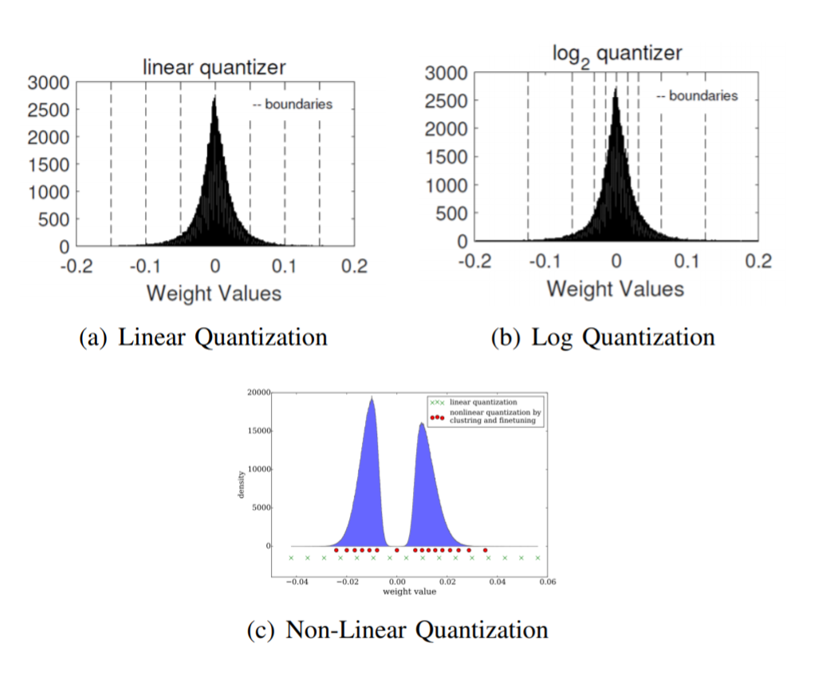
\includegraphics[width=0.8\linewidth]{inc/2_related_work/figure/quantization_types.png}
    \caption{Various methods of quantization from \cite{lognet}\cite{DeepCompression}}
    \label{fig:quant_types}
\end{figure}
\subsection{fixed point quantisation}
More related to this work, researches find the numerical requirement for even the latest DNN model inference stage far from the commonly used 32/64 bit floating-point format. \cite{FixedPoint} quantize the models to fixed point with ${L_2}$ error minimization, achieved \textbf{0.89\%} MCR (miss classification rate) on \textbf{MNIST} with 5 bits weights in comparison to \textbf{0.81\%} MCR with floating point weights.
\subsection{ternary to binary quantisation}
Some researchers have tried extreme quantization down to 2bits tenary weights such as in TWNs\cite{Ternary} and even binary weights in BinaryNet \cite{BinaryNet}, to binarize both weight and activation as in XNOR-net\cite{XnorNet}. \\
TWNs minimizes the Euclidian distance between the full precision weights $\boldsymbol{W}$ and tenary-valued weights $\boldsymbol{W^t}$ along with a non-negative scaling factor $\alpha$ in \eqref{eq:twn} achieving \textbf{99.35\%}, \textbf{92.56\%}, \textbf{84.2\%} on \textbf{MNIST}, \textbf{CIFAR-10}, \textbf{ImageNet(top-5)} dataset respectively.  
\begin{equation}
\begin{aligned}\label{eq:twn}
    \alpha^*, \boldsymbol{W^{t*}} = \mathop{\arg\min}_{\alpha,\boldsymbol{W^t}} = \|\boldsymbol{W}-\alpha\boldsymbol{W^t}\|^2_2 \\  
\text{s.t }\alpha\geq0,\boldsymbol{W^t_i}\in\{1,0,-1\}, i=1,2,...,n.
\end{aligned}
\end{equation}
BinaryNet constrains both weights and activations to either +1 or -1 with 
\begin{equation}
    \begin{aligned}\label{eq:bn}
        x^b=\text{Sign}(x)=\begin{cases}
                        +1 &\text{if \(x\geq0\)}, \\
                        -1 &\text{otherwise},
                    \end{cases}
    \end{aligned}
\end{equation}
achieving \textbf{0.96\%} , \textbf{10.15\%} error rate on \textbf{MNIST} , \textbf{CIFAR-10} dataset respectively.
And finally the Xnor-net put their emphasis on the scaling factor $\alpha^*$ and $\boldsymbol{K}$ between layers that first computes the floating point value of an output tensor, then take the sign of it for the binarized activation for the input of next layer.
\begin{equation}
    \begin{aligned}\label{eq:xnornet}
        \alpha^*=\frac{\boldsymbol{W^T}\text{sign ($\boldsymbol{W}$)}}{n}=\frac{\Sigma\|\boldsymbol{W_i}\|}{n}=\frac{1}{n}\|\boldsymbol{W}\|_{l1} \\
        \boldsymbol{K}=\frac{\Sigma\|\boldsymbol{I}_{:,:,i}\|}{c} * \frac{1}{w \times h}
    \end{aligned}
\end{equation}
In a Xnor-net particularly the convolutional operation seen in \figref{xnor_operation} can be appriximated by:
\begin{equation}
    \begin{aligned}\label{eq:xnorop}
        \boldsymbol{I}*\boldsymbol{W}\approx(sign(\boldsymbol{I}) * sign(\boldsymbol{W}))\odot\boldsymbol{K}\alpha
    \end{aligned}
\end{equation}
where $\boldsymbol{I}$, $\boldsymbol{W}$ denotes the input, weight tensors of a layer. Additionally, they discovered that regular batch-normalization layer position between convolution and activation function is unfriendly to binarization algorithm, by moving convolution layer after the activation function instead further boost the accuracy, achieving \textbf{69.2\%} top-5 accuracy on \textbf{ImageNet} using \textbf{AlexNet} model. By adopting binarization scheme, XNOR and bitcount operations can be applied to save computational cost at inference stage, with ~\textbf{58x} reported speed up against CPU time. \\
Pushing the limit to binarization hurts the accuracy by a large margin, worth mentioning that in Xnor-net they didn't quantize the first and the last layer of the convolution, which bear too much information to be discarded.
\begin{figure}
    \centering
    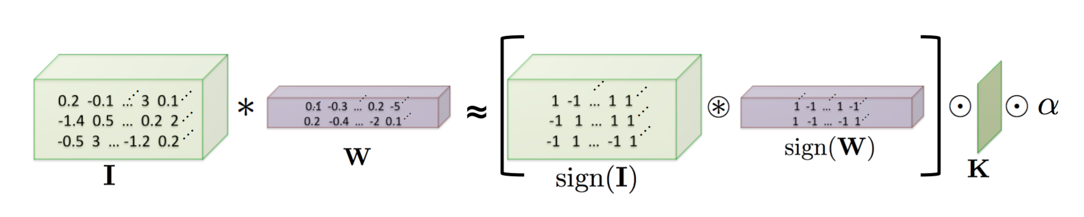
\includegraphics[width=0.8\linewidth]{inc/2_related_work/figure/xnor_operation.png}
    \caption{Convolution with XNOR-Bitcount in XNOR-net from \cite{XnorNet}}
    \label{fig:xnor_operation}
\end{figure}
 
\subsection{8-bit quantization on modern models}
More practically, modern deep models have been showed to work on 8 bits quantization on both weights and activations \cite{TensorRT8bit}. Taking advantage of Nvidia's bulit-in INT8 operations on their GPUs, they developed a CUDA library in TensorRT with an algorithm minimizing loss of information when quantizing trained model without further fine tunning or retraining. Starting with the tensor approximation with quantized tensor:
\begin{equation}
    \begin{aligned}\label{eq:tensorrtop}
    \textbf{Tensor Values}\approx\textbf{FP32 scaling factor}*\textbf{INT8 array}
    \end{aligned}
\end{equation}
 The scaling factor determines the mapping of the quantized level to the original value, for example a scaling factor of $\frac{2.7}{127}$ maps the quantized data 127 to original data 2.7. This is always a trade-off process between range and precision: the larger the scaling is, the larger the range, and the smaller the precision. The scaling process also includes the clipping of data exceeding a pre-defined threshold as seen in \figref{tensorrt_thresold}, and the threshold is in fact the scaling factor times the maximum level of the quantization, which is 127 in INT8 case.
\begin{figure}
    \centering
    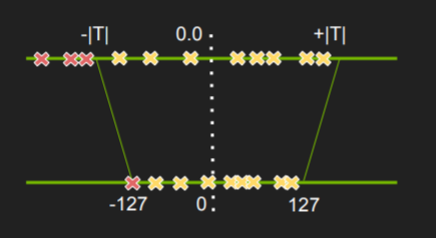
\includegraphics[width=0.5\linewidth]{inc/2_related_work/figure/tensorrt_thresold.png}
    \caption{Information loss is minimized through careful choice of saturation thresold from \cite{TensorRT8bit}}
    \label{fig:tensorrt_thresold}
\end{figure}
\\
Therefore the main challenge here is the choice of the scaling factor.As stated in the work, INT8 model encodes the same information as the original FP32 model, the choosing of the scaling factor is a process of minimizing the loss of information, which can be measured by Kullback-Leibler divergence as the relative entropy or information divergence \eqref{eq:kl_div}. They propose a \textbf{Calibration Dataset} to be run on FP32 format inference, collecting histograms of activations, and then pick thresold that minimize the KL divergence by generating many quantized data distributions with different saturation thresholds. This process is said to take only a few minutes on a desktop workstation. \\ 
\begin{equation}
    \begin{aligned}\label{eq:kl_div}
    \textbf{KL\_Divergence} ( \boldsymbol{P} , \boldsymbol{Q} ) := \textbf{SUM} ( \boldsymbol{P[i]} * log ( \frac{ \boldsymbol{P[i]}}{\boldsymbol{Q[i]}} ) , i)
    \end{aligned}
\end{equation}
The resulting INT8 model achieves no more than \textbf{0.46\%} extra error rate if even not lesser, at the same time speeding up from \textbf{1.62x} to \textbf{3.67x} depending on the inference batch size ( from 1 to 128) on their processor DRIVE PX2, dGPU.
In \autoref{ch:low prec NN} we propose a similar yet simpler scheme to compute the desirable quantization threshold, although our approach involves no calibration after the training, the re-training process is working in low-precision condition and is much slower than train-then-fine-tune scheme in this work. However, we believe that re-training on ultra-low-precision model ( $<$ 8 bits) is still necessary.

\section{Hardware design}
Recently researches related to deep neural network accelerator are blooming rapidly. They typically start off with a core algorithm simplifying the NN model, then combining either micro-architectural optimization such as low-precision arithmetic units or system level optimization involving data compression between the chip and the off-chip memory, delicate buffer design, sparsity-aware zero-skipping operations and so on. \\
We are going to focus on several works that inspire us the most, including modified classic systolic-array style processor operating on a granularity of rows, SIMD (single instruction multiple data) style processor coupled with re-configurable arithmetic unit being able to operate on 1-16 bits respectively.
From these works, we conclude that slashing down memory access counts either from on-chip or off-chip is of upmost importance for chip power efficiency, through further low-bit operation optimization the memory transaction frequency can be furthered improved. 
\subsection{Dataflow optimization: row stationary}
Eyeriss\cite{Eyeriss} analyzes existing accelerator work in a now widely used manner, classifying them into \textit{Weight Stationary}, \textit{Output Stationary}, \textit{No Local Reuse} three dataflows that reuse data differently, and propose a novel processing dataflow coined \textit{Row Stationary}. 
\subsection{Sub-word parallelism arithmetic unit}
\subsection{Bit-level re-configurable arithmetic unit}
\begin{itemize}
    \item \textcolor{purple}{How does related work "relate" to your research question?}
    \item \textcolor{purple}{Does it provide a starting point?}
    \item \textcolor{purple}{Does it provide evidence that you are posing a good research question?}
    \item \textcolor{purple}{Does it provide a different approach to a similar research hypothesis that you can compare to?}
\end{itemize}
\chapter{Low numeric precision convolution neural network}
\label{ch:low prec NN}


In this chapter, we go through the basic of convolution neural network, the mindset behind choosing linear quantization scheme, an algorithm for training a ultra-low precision neural network on large-scale dataset and finally a tensor re-pack method for deploying the network on a processor supporting low-precision MAC operation.
\section{Convolutional Neural Networks}
A typical convolution neural network layer takes a 3D \textit{input tensor} and a \textit{filter tensor}, and performs 2D convolution, producing a 3D \textit{output tensor}.It is essentially summing up \textbf{C} channel of 2D convolution for one output pixel as shown in \autoref{fig:conv_1}, this process is repeated for \textbf{M} number of filter, resulting in output tensor of \textbf{M} number of channel. 
In \autoref{fig:conv_2} shows a common techniques \textit{batching}, taking multiple input tensor and perform convolution on them at the same time; the picture also provides an example of the shape parameter \textbf{U}.
\begin{figure}
    \centering
    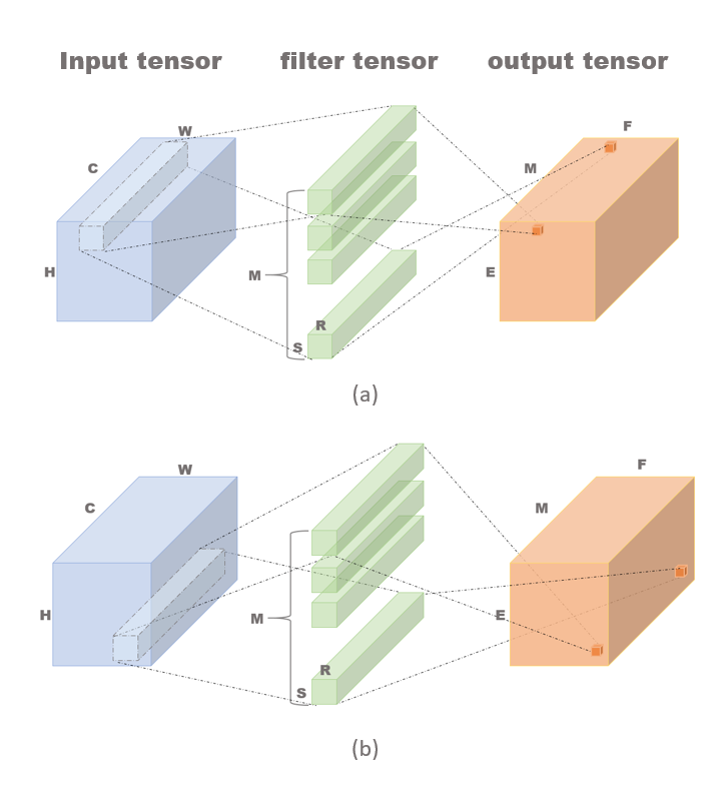
\includegraphics[width=1\linewidth]{inc/3_low_numeric_convolution_neural_network/figure/convolution_1.png}
    \caption{Computation of a convolutional layer.}
    \label{fig:conv_1}
\end{figure}
\begin{figure}
    \centering
    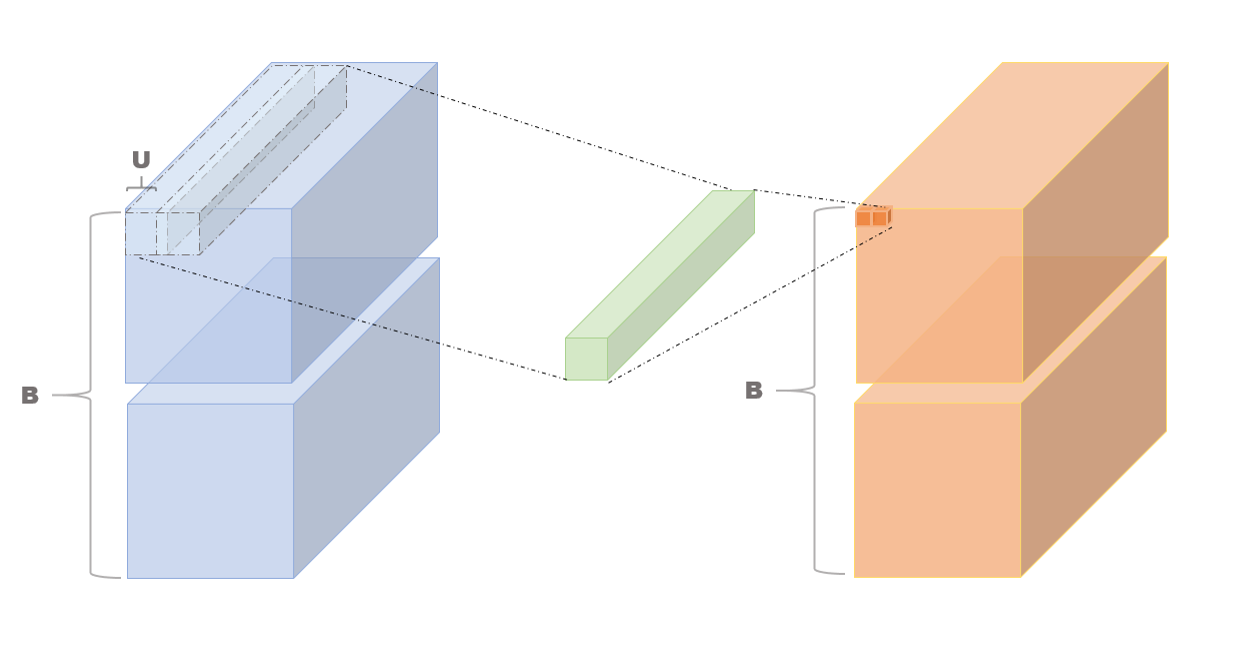
\includegraphics[width=1\linewidth]{inc/3_low_numeric_convolution_neural_network/figure/convolution_2.png}
    \caption{Shape parameter B and U.}
    \label{fig:conv_2}
\end{figure}
The entire process is formulated by \autoref{eq:conv}:
\begin{equation}
    \begin{aligned}\label{eq:conv}
    \boldsymbol{O}[z][u][x][y]=\text{ReLU}\,(
        \sum^{C-1}_{k=0}\sum^{R-1}_{i=0}\sum^{S-1}_{j=0}\boldsymbol{I}[z][k][Ux+i][Uy+j]*\boldsymbol{W}[u][k][i][j]
    ), \\
    0\leq z\leq B\ , 0\leq u\leq M\ , 0\leq y\leq E\ , 0\leq x\leq F, \\
    E=(H-R+U)/U,\,F=(W-S+U)/U
    \end{aligned}
\end{equation}


\begin{table}
    \caption{Basic shape parameters of a CNN layer}
    \label{tab:cnn_shape}
    \centering
    \footnotesize 
        \begin{tabular}{cc}
        \toprule
        Parameter & Description \\
        \midrule
        H/W & Input feature map spatial dimensions\\
        E/F & Output feature map spatial dimensions\\
        R/S & Filter spatial dimensions\\
        C & Input channels\\
        M & Output filters\\
        U & Convolution stride\\
        B & Batch,\# of feature maps to be processed\\
        \bottomrule
        \end{tabular}
\end{table}


 
\section{Low Precision CNN}
By choosing linear quantization regular multiplier and adder can be used unlike the need of look-up table in non-linear quantization. As mention briefly before, the main benefit of quantization is reduction in memory transaction, especially off-chip DRAM access. We will show in \autoref{ch:results} that given the same dataflow, 8-bit quantized model off-chip memory access wins over 16-bit model compressed with \textit{running length coding} with data sparsity of more than 70\%, indicating that quantization is a reliable compression scheme independent of sparsity of the data. This sums up our reasons behind choosing linear quantization. \\
Low numeric precision data in this work is applied to each type of tensors. Given a quantization bit $\boldsymbol{k}$, clipping threshold $\boldsymbol{\tau}$, tensor $\boldsymbol{D}$, the quantized tensor $\boldsymbol{D_q}$ is given by \autoref{eq:quant}:
\begin{equation}
    \begin{aligned}\label{eq:quant}
        \boldsymbol{D_q}=
        \textit{round}\ (\ \frac{2^{\boldsymbol{k}-1}}{\boldsymbol{\tau}}*\textit{clip}\ (\boldsymbol{D},\boldsymbol{\tau})
        \ ) \\
        \textit{clip}(\boldsymbol{D},\boldsymbol{\tau})=\begin{cases}
            \boldsymbol{D} &\|\boldsymbol{D}\|<\boldsymbol{\tau} \\
            \textit{sign}(\boldsymbol{D})*\boldsymbol{\tau} &\text{otherwise}
        \end{cases} \\
    \end{aligned}
\end{equation}
Where \textit{round}() round the number to the nearest integer. The convolution on the original tensor can therefore take the following form \autoref{eq:quant_conv}:
\begin{equation}
    \begin{aligned}\label{eq:quant_conv}
        \boldsymbol{O}\approx\boldsymbol{I}\star\boldsymbol{W}= \boldsymbol{I_q}\star\boldsymbol{W_q}
        \ \frac{\boldsymbol{\tau_I}}{2^{k_I-1}}
        \ \frac{\boldsymbol{\tau_W}}{2^{k_W-1}}
        =\boldsymbol{O_q}\  \frac{\boldsymbol{\tau_O}}{2^{k_O-1}} \\
        \boldsymbol{\alpha}\boldsymbol{I_q}\star\boldsymbol{W_q}=\boldsymbol{O_q}
    \end{aligned}
\end{equation}
\begin{equation}
    \begin{aligned}\label{eq:scalar_approx}
        \boldsymbol{\delta}=\textit{ round} ( log_2\alpha)\quad
        \boldsymbol{\gamma}=\textit{ round}( \frac{\alpha}{2^{\delta}})\quad
        \boldsymbol{\alpha}\approx=\delta\gg\gamma
    \end{aligned}    
\end{equation}
We see the part $\boldsymbol{I_q}\star\boldsymbol{W_q}$ is the low precision convolution fit for specially designed processor. $\boldsymbol{\alpha}$ merges the rest of the equation to a scaling factor, which in practice can be approximated together with other scaling factor with a 16-bit fixed-point multiplier $\boldsymbol{\delta}$ and a shifting factor $\boldsymbol{\gamma}$, see \autoref{eq:scalar_approx}. \\
The training of low precision neural network follows that of \cite{XnorNet}. See \autoref{alg:NN_train}; at training, the quantized convolution results are fed forward through the network, error is computed based on the quantized value, and the gradient is back-propagated bypassing the quantization steps, updating the full-precision weights.
\begin{algorithm}
    \SetAlgoLined
        $\boldsymbol{O}=\textbf{QuantForward}(\boldsymbol{I_q},\boldsymbol{W_q},\boldsymbol{\tau_I},\boldsymbol{\tau_W},k_W,k_I )$ \\
        $\frac{\partial \boldsymbol{C} }{\partial \boldsymbol{W}}$
        \text{=\ }\textbf{QuantBackward}\text{(\ }  $\frac{\partial\boldsymbol{C}}{\partial\boldsymbol{O}}$
        \text{$,\boldsymbol{W_q})$} 
        // the gradient is caculated based on the quantized weight \\
        $\boldsymbol{W^{t+1}}=\textbf{UpdateParameters}(\boldsymbol{W^t},\ $ $\frac{\partial\boldsymbol{C}}{\partial\boldsymbol{W}})$ 
        // real gradient is replaced by that from quantized weight, bypassing the quantization function
    \caption{quantization NN training}
    \label{alg:NN_train}
\end{algorithm}

\section{Quantization Loss Minimization Threshold Selection}
We propose a simple algorithm for quantization threshold choosing. \textit{Batch Normalization} layer \cite{BatchNormalization} has been widely used in modern NN models, speeding up the convergence process and possibly improve the accuracy. The layer introduce additional scaling factor and bias base on input data distribution along the batch, it helps the \textit{internal covariate shift} phenomena, so that non-linearity layers take effect more reliably. Simply put, the scaling and bias calibrate the output to have a mean of 0 and variance of 1, and naturally, it is heuristic to model the distribution with a \textit{standard normal distribution}. With the assumption that our data are of standard normal distribution, given a target quantization bit, we would generate a large number of data of standard normal distribution, iterate over a set of threshold selection, and pick the threshold posing the least quantization error, the error is either calculated with \textit{$L_1$} norm or \textit{$L_2$} norm. The thresholds for each quantization bits are then fixed and applied throughout the entire model. We tested the impact of error calculation on model accuracy and choose \textit{$L_1$} norm. 

\begin{algorithm}
    \SetAlgoLined
    \caption{quantization threshold selection}
    \label{alg:th_choice}
    \begin{algorithmic}[1]
        \REQUIRE{$k,\boldsymbol{\tau}$} \\
        \ENSURE{$\tau$} \\
        generate \boldsymbol{D} array of standard normal distribution array\\
        \FOR{each item $\tau_i$ in $\boldsymbol{\tau}$}
            \STATE{$\boldsymbol{D_q}=round\ (\ \frac{2^{k-1}}{\tau_i}\ clip\ (\boldsymbol{D},\tau_i)\ )$}
            \STATE{$\boldsymbol{D_r}=\boldsymbol{D_q}*\frac{\tau_i}{2^{k-1}}$} 
            \STATE{$\boldsymbol{E_{1i}}=\Sigma\|\boldsymbol{D}-\boldsymbol{D_r}\|$}
        \ENDFOR
        \RETURN{$\tau_i=\underset{\tau_i}{\operatorname{argmin}} \boldsymbol{E_1}(\tau_i)$}
    \end{algorithmic}
\end{algorithm}
\begin{figure}
    \centering
    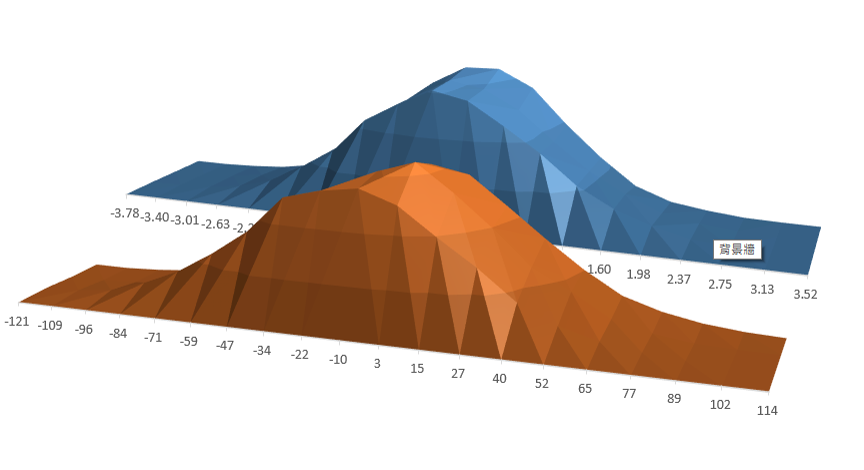
\includegraphics[width=1\linewidth]{inc/3_low_numeric_convolution_neural_network/figure/nor_dist.png}
    \caption{Given a threshold, calculate the error between reconstructed distribution and the original.}
    \label{fig:th_choice}
\end{figure}
\begin{table}[h]
    \caption{Threshold for each bit setting by $L_1$ norm error}
    \label{tab:threshold}
    \centering
    \footnotesize 
        \begin{tabular}{c|ccccccccc}
        \toprule
            Bit length &1 & 2 & 3 & 4 & 5 & 6 & 7 & 8 & 32 \\
            Threshold &1.2 & 1.9& 2.4& 2.7& 3.1& 3.5& 3.6& 3.7& 100 \\
 
        \bottomrule
        \end{tabular}
\end{table}

\section{Computational consideration and data re-packing}
Now that we have the quantized model, we need efficient computational strategy. Simply store the model, say quantized to 4 bits, in original 32-bit data type is 8x waste of storage, memory bandwidth and can't be effectively deployed to processing unit. We propose a simple data re-packing method, to tightly compact the data. However the compacted data requires specially designed processor to reach its full performance potential. Since we're aiming at large image recognition task, the data usually can't fit onto the accelerator entirely. We use several tiling parameters to split data into chunks and process them one at a time.
\subsection{Data re-packing}
We first determine a desirable MAC bit-length configuration \textbf{$A_b$}, usually the smaller bit-length of input and weight tensor. We then split each data point and distribute them to an additional tensor dimension \textit{bit channel} if the data bit-length is larger than \textbf{$A_b$}, \textbf{$X_b,W_b,O_b$} for input, weight, output respectively, note that \textbf{$O_b$} is dependent on the \textbf{$A'_b$} of the next layer. Say we are going to process a layer using 4-bit multiplication, \textbf{$A_b$} is chosen to be 4; in \autoref{fig:re_pack1}, original 4-bit data stored in wasteful 16-bit is re-packed along the \textbf{channel} dimension into new channel size of $C/4$; \autoref{fig:re_pack2} re-packs 8-bit data with additional \textbf{$X_b$} dimension of size 2.The re-packed data is meant to be added up within itself, and the data with different \textit{bit channel} bear different weighting of $2^{X_b*A_b}$. In the example, we need a arithmetic unit capable of summing up 4 4-bit multiplication within a 16-bit data, we call this \textbf{\textit{subword accumulation}} arithmetic dataflow, in contrast to the \textit{subword parallelism} dataflow where multiple output registers are needed, only one output register is needed at a time. We will elaborate in \autoref{ch:arch}.
\\
Having the data prepared through quantization and re-packing, we are ready to move on to the accelerator architecture designed for such data.
\begin{figure}
    \centering
    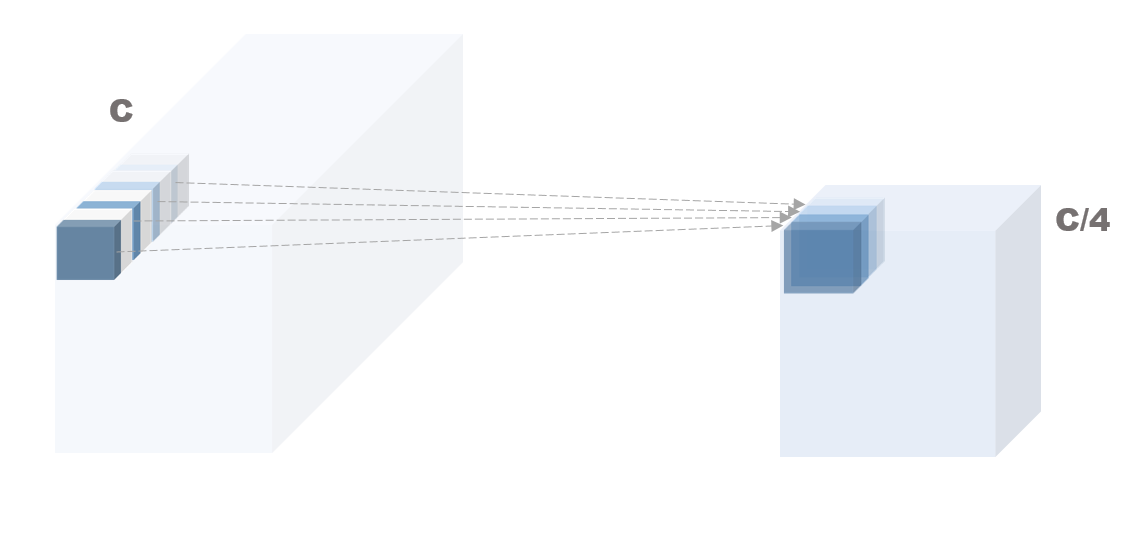
\includegraphics[width=1\linewidth]{inc/3_low_numeric_convolution_neural_network/figure/re_pack1.png}
    \caption{4-bit data repacked to 16-bit compact data.}
    \label{fig:re_pack1}
\end{figure}
\begin{figure}[h]
    \centering
    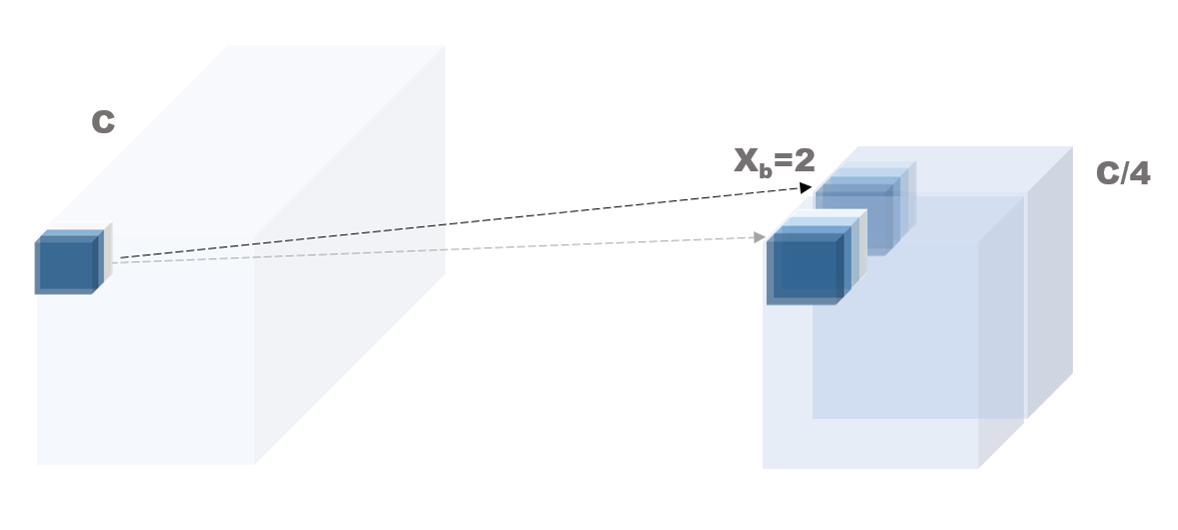
\includegraphics[width=1\linewidth]{inc/3_low_numeric_convolution_neural_network/figure/re_pack2.png}
    \caption{8-bit data repacked to 16-bit compact data with additional bit channel data of size 2.}
    \label{fig:re_pack2}
\end{figure}
\begin{table}[h]
    \caption{Low bit arithmetic and shape parameters}
    \label{tab:bit_shape}
    \centering
    \footnotesize 
        \begin{tabular}{cc}
        \toprule
        Parameter & Description \\
        \midrule
        $X_b$ & Input bit channels\\
        $W_b$ & Weight bit channels\\
        $O_b$ & Output bit length\\
        $A_b$ & Arithmetic bit length\\
        $A'_b$ & Arithmetic bit length of the next layer\\
        \bottomrule
        \end{tabular}
\end{table}


\iffalse
    \begin{itemize}
    \textcolor{purple}{What knowledge is necessary to}
        \item \textcolor{purple}{understand design decisions you made, e.g. how did you choose the quantisation     algorithm?}
        \item \textcolor{purple}{understand why your research question is important, e.g. why should we quantise     CNNs?}
    \end{itemize}
\fi
\chapter{Proposed Architecture}
The architecture design is targeted to capture as much data reuse as possible, a three-level hierarchy on-chip buffer exploits almost every data reuseability in a regular convolution layer in the mean time saving power by logistically decreasing buffer size: data stay longer in the lower and smaller hierarchy buffer. As parallelism goes up, memory dispatching to each PE is not a task regarding bandwidth, but a huge burden to the control logic; with data rearrangement, we can efficiently transfer data between buffer and buffer, or buffer and PE with shifter instead of MUX, saving logic and potentially power. Finally we propose three micro-architecture dedicated to low-bit multiplication adder tree, able to operate on 1,2,4,8 bits signed and unsigned data, and an additional XNOR functionality\TODO{final choice}.
\textcolor{purple}{This chapter is your proof. You have shown in the previous chapters what the starting point is and why it is important to advance. This chapter describes how you advance and how you made choices. It also shows what (performance) results your choices lead to. Ideally, it identifies how certain choices influence the final performance.}
\section{System Overview}
\subsection{Dataflow}
\subsection{Buffer hierarchy}
\section{Architecture Overview}
\subsection{PE processing pipeline}
\subsection{Re-configurable arithmetic logic unit}
\subsection{Partial sum propagate path}
\subsection{Data dispatch shifter}

\chapter{Results}
\label{ch:results}
\section{Quantization error minimization training}
Our quantization error minimization training on AlexNet achieves $54\%$ accuracy with the following setting in \autoref{tab:alex_train}. Note that we apply quantization on the first layer as well, and some of the model shape doesn't follow a typical AlexNet model. The input bit-length stays 8-bit as original. \autoref{tab:acc_comp} shows the classification accuracy of several works on ImageNet using AlexNet, note that the first layer of XNOR-net is not quantized, and possibly pose a large computational overhead over quantized one. 
\begin{table}[h]
    \caption{AlexNet 4-bit quantization}
    \label{tab:alex_train}
    \centering
    \footnotesize 
        \begin{tabular}{c|cccccccc}
        \toprule
        layer & conv1 & conv2 & conv3 & conv4 & conv5 & Fc1 & Fc2 & Fc3\\
        \midrule
        Weight & 4 & 4 & 4 & 4 & 4 & 2 & 2 & 32 \\
        Activation & 4 & 4 & 4 & 4 & 4 & 4 & 4 &32\\
        Output channels & 64 & 256 & 256 & 256 & 256 & 4096 & 4096 & 1000\\
        \bottomrule
        \end{tabular}
\end{table}
\begin{table}[h]
    \caption{Classification Accuracy on ImageNet, AlexNet}
    \label{tab:acc_comp}
    \centering
    \footnotesize 
        \begin{tabular}{c|c|c|c|}
        \toprule
        &XNOR-Net\cite{XnorNet} & TensorRT\cite{TensorRT8bit} & OUR\\ 
        \midrule
        Bit-length & 1& 8 & 4 \\
        Accuracy & 44.2\% & 57\% & 54\%\\
        \bottomrule
        \end{tabular}
\end{table}
\section{Implementation results}
We synthesize and evaluate our design using TSMC 90nm technology. The PE array and Buffer specification is provided in \autoref{tab:spec}, the best synthesized cell area is 15698896 cell area, approximately 15.6 $mm^2$. We co-simulate the design using \textbf{Nicotb}\cite{nicotb} and Cadence nc-verilog version 15.20-s039; we synthesize the design with Synopsys design compiler version 0-2018.06 and finally simulate power consumption with Synopsys PrimeTime version M-2017.06-SP2. \autoref{tab:comp} lists several highly related hardware implementation works in comparison, note that Vgg16 benchmark setting is not yet trained on 4-bit arithmetic setting, yet we are highly confident that there is room for quantization for such redundant network. \\
\begin{table}[h]
    \caption{System specification}
    \label{tab:spec}
    \centering
    \footnotesize 
        \begin{tabular}{c|c}
        \toprule
        \midrule
        Technology & TSMC 90nm GUTM Arm f1.0\\
        Gate count (logic only) & 1340.7k (NAND2)\\
        Area & 15.6$mm^2$\\
        PE dimension & 16x16\\
        On-chip SRAM & 124KB\\
        Register file & 56K+384B\\
        Clock rate & 200-400MHz\\
        Peak throughput & 51.2N-102.4N GOPs, N=16,8,4,2\\
        Arithmetic precision & re-configurable 1,2,4,8-bit fixed-point\\
        Average full power & 672mW @200MHz\\
        Power efficiency & 76.19N-152.38N GOPs/W, N=16,8,4,2\\
        \bottomrule
        \end{tabular}
\end{table}
\begin{table}[h]
    \caption{System specification comparison.}
    \label{tab:comp}
    \centering
    \footnotesize 
        \resizebox{\linewidth}{!}{%
        \begin{tabular}{c|cccc}
        \toprule
        Work & JSSC'17\cite{Eyeriss} & ISSCC'17\cite{ENVISION} & VLSI'16\cite{PrecisionScalableVLSI}    & This work N=16,8,4,2\\
        \midrule
        Technology & 65nm LP CMOS & 40 LP CMOS & 28nm UTBB FD-SOI & 90nm CMOS\\
        Tape-out  & V & V & V & pre-sim\\
        \midrule
        Frequency & 200 & 200 & 200 & 400\\
        Supply voltage  & 1 & 1.1 & 1 & 1\\
        Peak GOPs& 67 & 102 & nx102 n=1,2,4 & Nx152.38 \\
        \midrule
        Area $(mm^2)$ & 12.25 & 2.4 & 1.87 & 15.6\\
        \# of MACs & 168 & 256 & nx256 n=1,2,4 & Nx256\\
        Gate Counts & 1.176M &  1.6M & 1.95M & 1.34M\\
        On-chip memory (KB) & 184.5 & 144 & 144 & 180\\
        \midrule
        Precision & 16-bit fixed & Dynamic 1-16 & Dynamic Nx 1-16/N & 1,2,4,8\\
        \midrule
        AlexNet benchmark & 278mW @34.7fps &  76mW @ & 20-62, 44mW @47fps & 506mW avg @206.9fps,4b\\
        Vgg16 benchmark & 236mW @0.7fps & - & 26mW @1.67fps & 586mW @ 6.86fps,4b,N/A acc\\
        
        \bottomrule
        \end{tabular} }
\end{table}

\subsection{Area and power}
\autoref{fig:area_breakdown} shows the area breakdown chart for this work, PE logic takes up 25\% of area in contrast to $75\%$ of memory, which actually accounts for a large portion in comparison to related work, as multipliers in \cite{Eyeriss} takes up $7.4\%$ of area. 
\begin{figure}[h]
    \centering
    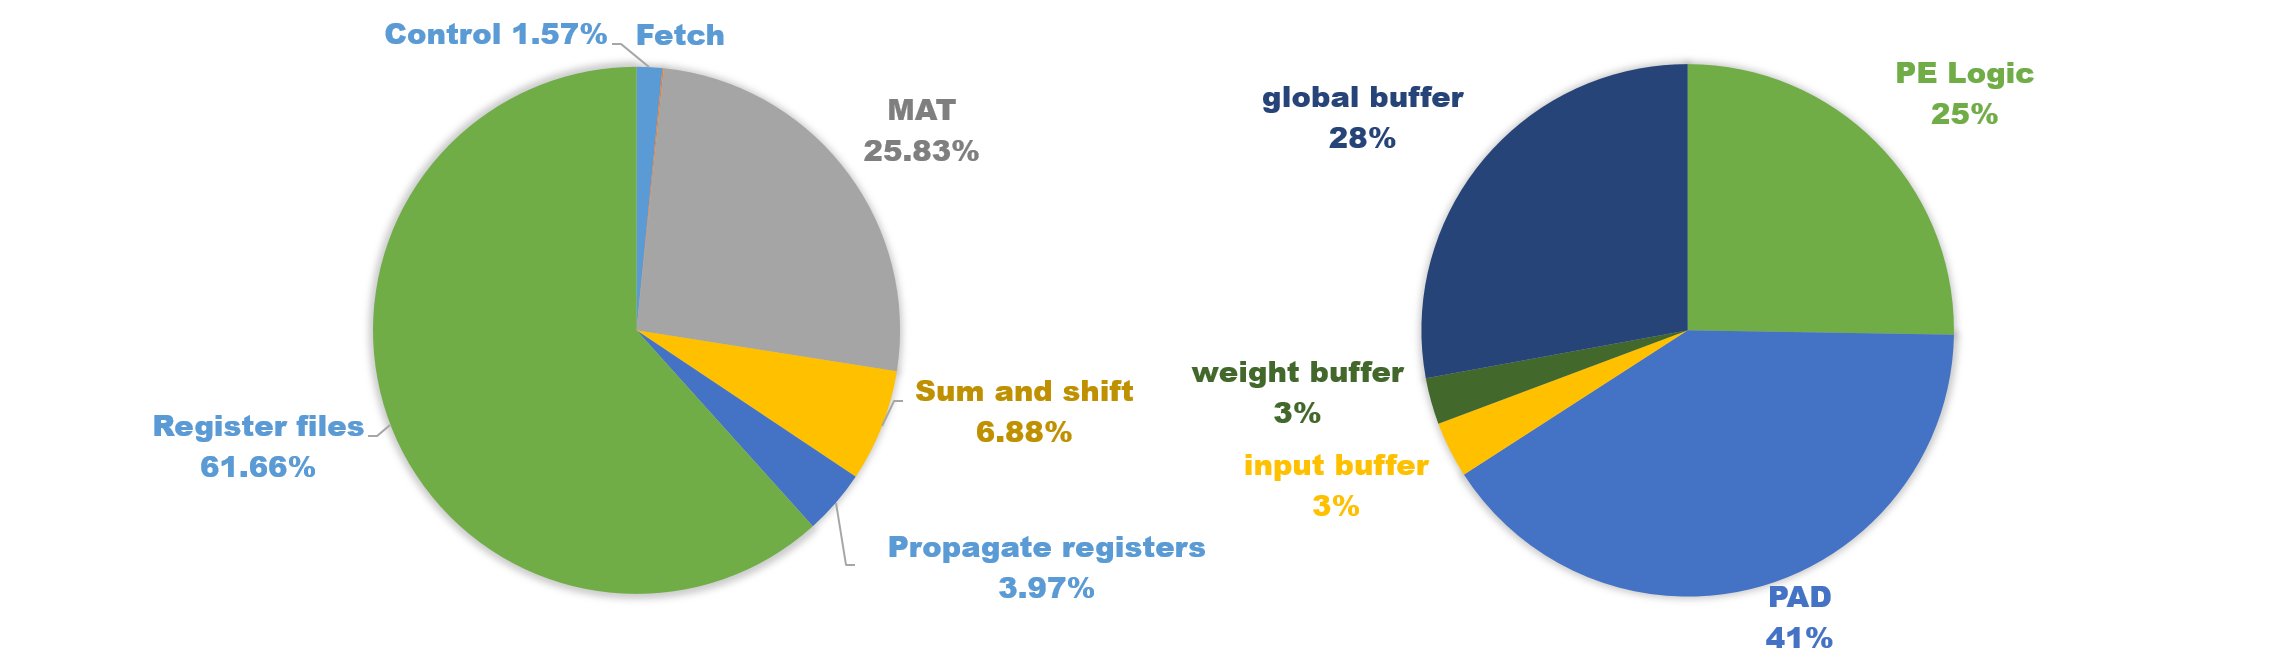
\includegraphics[width=1\linewidth]{inc/5_results/figure/area_breakdown.png}
    \caption{Area breakdown of the system.}
    \label{fig:area_breakdown}
\end{figure}
\begin{table}[h]
    \caption{PE column area gate counts}
    \label{tab:area_gate}
    \centering
    \footnotesize 
        \begin{tabular}{clccccccc}
        \toprule
        control  & Fetch  & MAT       & Sum and shift       & Propagator      & IPAD     & PPAD     & WPAD    & total       \\
        \midrule
        3670 & 200 & 60503 & 16122 & 9295 & 2756 & 74856 & 66802 & 234207\\
        \bottomrule
        \end{tabular}
\end{table}
\autoref{fig:buffer_hier} shows the buffer hierarchy significance, removing input and weight buffer introduces a $1.14$x power consumption overhead on representative AlexNet conv5 layer. The additional buffer takes up about $20\%$ more area as a trade-off. 
\begin{figure}[h]
    \centering
    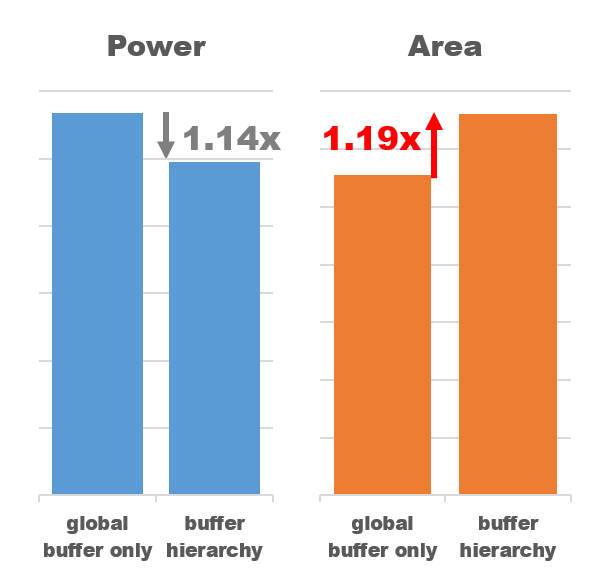
\includegraphics[width=0.6\linewidth]{inc/5_results/figure/buffer_hier.png}
    \caption{Buffer hierarchy area power trade-off.}
    \label{fig:buffer_hier}
\end{figure}
\autoref{fig:power_breakdown} shows the power breakdown of the system. The PE array consumes most portion of the power, indicating workloads falls mainly on the most power efficient part of the system. The PAD access, MAT, sum and shift draws close amount of power. \autoref{tab:power} shows a 4-bit layer power consumption simulated at 200MHz, 1V. \autoref{fig:operation_power} shows the power consumption of different bit mode setting on MAT, indicating that the low-precision operations contributes mainly on memory access saving, the system benefits from arithmetic operation lightly.
\begin{figure}[h]
    \centering
    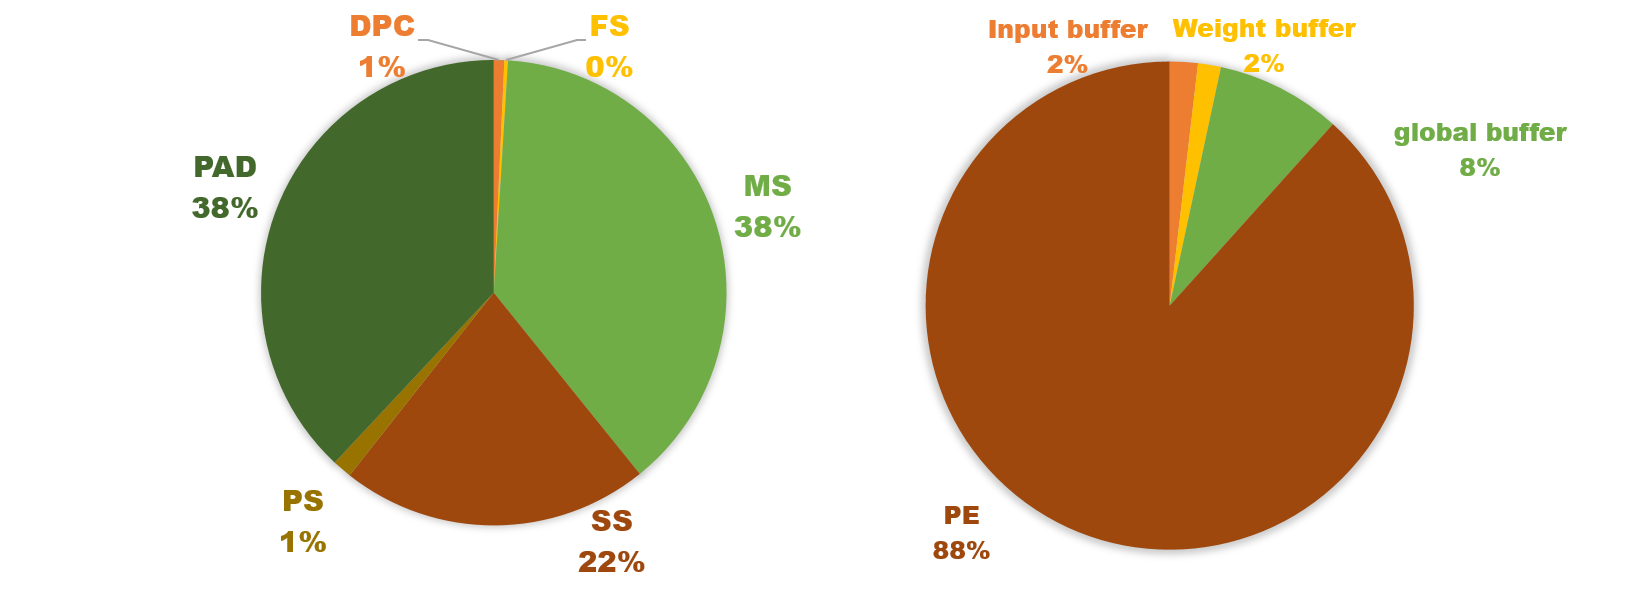
\includegraphics[width=1\linewidth]{inc/5_results/figure/power_breakdown.png}
    \caption{Average power breakdown of the system.}
    \label{fig:power_breakdown}
\end{figure}

\begin{figure}
    \centering
    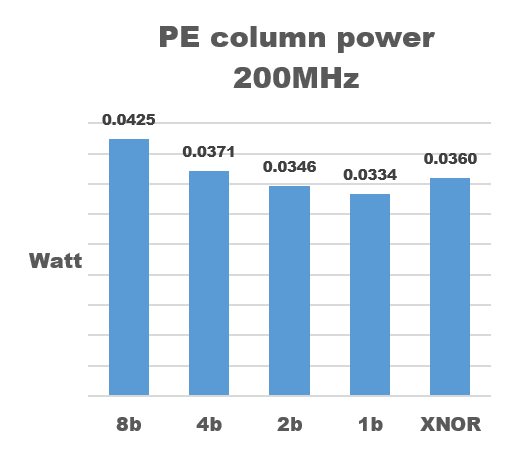
\includegraphics[width=0.6\linewidth]{inc/5_results/figure/operation_power.png}
    \caption{Arithmetic unit configuration power.}
    \label{fig:operation_power}
\end{figure}
\begin{table}[h]
    \caption{System average power (mW) consumption at 200MHz}
    \label{tab:power}
    \centering
    \footnotesize 
        \begin{tabular}{cccccccc}
        DPC  & FS   & MS    & SS     & PS   & PAD     & buffer hierarchy & total   \\
        \toprule
        4.16 & 1.44 & 219 & 122. & 7.68 & 218 & 79.1           & 652.5\\
        \bottomrule
        \end{tabular}
\end{table}






\subsection{Experiments} 
We lists the configuration and setting used on various models, and the performance reports. All the experiments set the batch size $B$ to 4, processes at 200MHz, 1V. Note the $psum word$ parameter is the partial sum word length storage on-chip, a word is of 16-bit, we use 2 word 32-bit for partial sum when overflow takes place frequently. Our hardware utilization rate is easily determined, which is usually $T_h$, the active PE column counts as well as the output rows processed in a PE row. If $T_h$ is larger than the PE column number 16, we allocate as much resource, as in PE columns as possible, and gated idle PE columns at the last height tile. For the most part, our hardware utilization rate on ImageNet, where the input spatial size is of 224x224, is usually $13/16(81.25\%)$. The utilization rate can be easily scaled up if we fit the design to a particular dataset spatial dimension, however we choose the PE shape for general purpose, and multiple of 16 is usually suitable for hardware designs. From various experiments we can see the power of quantization as low as to 4-bit, it boosts the processing time and reduce off-chip memory access even without coding or compression at the edge of the system. More importantly, the design is highly flexible and fit for various bit-length and model shapes. \\

\begin{table}[h]
    \caption{AlexNet configurations}
    \label{tab:alex_conf}
    \centering
    \footnotesize 
    \resizebox{\linewidth}{!}{%
        \begin{tabular}{l|lllllllllllllllllll}
                      & $T_w$ & $T_h$ & $H'$ & $W'$ & $P_{ch}$ & $X_b$ & $W_b$ & $A_b$ & $O_b$ & $P_m$ & $R$  & $S$  & $T_m$ & $T_b$ & $C$   & $E$  & $F$  & $M$   & psum word \\
                      \toprule
        alex conv1     & 14 & 14 & 63 & 63 & 1   & 2  & 1  & 4  & 4  & 2  & 11 & 11 & 64 & 2  & 3   & 55 & 55 & 64  & 2         \\
        alex conv2     & 27 & 27 & 31 & 31 & 2   & 1  & 1  & 4  & 4  & 2  & 5  & 5  & 64 & 1  & 64  & 27 & 27 & 256 & 1         \\
        alex conv3,4,5     & 13 & 13 & 15 & 15 & 4   & 1  & 1  & 4  & 4  & 4  & 3  & 3  & 64 & 4  & 256 & 13 & 13 & 256 & 1         \\
        old alex conv3 & 13 & 13 & 15 & 15 & 4   & 1  & 1  & 4  & 4  & 4  & 3  & 3  & 64 & 4  & 256 & 13 & 13 & 384 & 1         \\
        old alex conv4 & 13 & 13 & 15 & 15 & 4   & 1  & 1  & 4  & 4  & 4  & 3  & 3  & 64 & 4  & 192 & 13 & 13 & 384 & 1         \\
        old alex conv5 & 13 & 13 & 15 & 15 & 4   & 1  & 1  & 4  & 4  & 4  & 3  & 3  & 64 & 4  & 192 & 13 & 13 & 256 & 1         \\

        \bottomrule
        \end{tabular}
    }
\end{table}
\begin{table}[h]
    \caption{Vgg-16 configurations}
    \label{tab:vgg_conf}
    \centering
    \footnotesize 
    \resizebox{\linewidth}{!}{%
        \begin{tabular}{l|llllllllllllllllllllll}
                & $T_w$ & $T_h$ & $H'$ & $W'$ & $P_{ch}$ & $X_b$ & $W_b$ & $A_b$ & $O_b$ & $P_m$ & $R$  & $S$  & $T_m$ & $T_b$ & $C$   & $E$  & $F$  & $M$   & psum word \\
        \toprule
            vgg1   & 16 & 16 & 18 & 18 & 4   & 2  & 1  & 4  & 4  & 2  & 3 & 3 & 64 & 2  & 3   & 224 & 224 & 64  & 2         \\
            vgg1-2 & 16 & 16 & 18 & 18 & 4   & 1  & 1  & 4  & 4  & 4  & 3 & 3 & 64 & 4  & 64  & 224 & 224 & 64  & 1         \\
            vgg2-1 & 16 & 16 & 18 & 18 & 4   & 1  & 1  & 4  & 4  & 4  & 3 & 3 & 64 & 4  & 64  & 224 & 224 & 128 & 1         \\
            vgg2-2 & 16 & 16 & 18 & 18 & 4   & 1  & 1  & 4  & 4  & 4  & 3 & 3 & 64 & 4  & 128 & 112 & 112 & 128 & 1         \\
            vgg3-1 & 16 & 16 & 18 & 18 & 4   & 1  & 1  & 4  & 4  & 4  & 3 & 3 & 64 & 4  & 128 & 112 & 112 & 256 & 1         \\
            vgg3-2,3 & 16 & 16 & 18 & 18 & 4   & 1  & 1  & 4  & 4  & 4  & 3 & 3 & 64 & 4  & 256 & 56  & 56  & 256 & 1         \\
            vgg4-1 & 16 & 16 & 18 & 18 & 4   & 1  & 1  & 4  & 4  & 4  & 3 & 3 & 64 & 4  & 256 & 56  & 56  & 512 & 1         \\
            vgg4-2,3 & 16 & 16 & 18 & 18 & 4   & 1  & 1  & 4  & 4  & 4  & 3 & 3 & 64 & 4  & 512 & 28  & 28  & 512 & 1         \\
            vgg5-1 & 15 & 15 & 18 & 18 & 4   & 1  & 1  & 4  & 4  & 4  & 3 & 3 & 64 & 4  & 512 & 28  & 28  & 512 & 1         \\
            vgg5-2,3 & 14 & 14 & 18 & 18 & 4   & 1  & 1  & 4  & 4  & 4  & 3 & 3 & 64 & 4  & 512 & 14  & 14  & 512 & 1         \\

        \bottomrule
        \end{tabular}
    }
\end{table}

\begin{table}[h]
    \caption{XNOR AlexNet configurations}
    \label{tab:alex_conf}
    \centering
    \footnotesize 
    \resizebox{\linewidth}{!}{%
        \begin{tabular}{l|lllllllllllllllllll}
                      & $T_w$ & $T_h$ & $H'$ & $W'$ & $P_{ch}$ & $X_b$ & $W_b$ & $A_b$ & $O_b$ & $P_m$ & $R$  & $S$  & $T_m$ & $T_b$ & $C$   & $E$  & $F$  & $M$   & psum word \\
                      \toprule
            alexnor conv1     & 14 & 14 & 63 & 63 & 1   & 1  & 1  & 8  & 1  & 2  & 11 & 11 & 64 & 2  & 3   & 55 & 55 & 64  & 2         \\
            alexnor conv2     & 27 & 27 & 31 & 31 & 2   & 1  & 1  & 1  & 1  & 2  & 5  & 5  & 64 & 1  & 64  & 27 & 27 & 256 & 1         \\
            alexnor conv3 & 13 & 13 & 15 & 15 & 4   & 1  & 1  & 1  & 1  & 4  & 3  & 3  & 96 & 4  & 256 & 13 & 13 & 384 & 1         \\
            alexnor conv4 & 13 & 13 & 15 & 15 & 4   & 1  & 1  & 1  & 1  & 4  & 3  & 3  & 96 & 4  & 192 & 13 & 13 & 384 & 1         \\
            alexnor conv5 & 13 & 13 & 15 & 15 & 4   & 1  & 1  & 1  & 1  & 4  & 3  & 3  & 96 & 4  & 192 & 13 & 13 & 256 & 1       \\

        \bottomrule
        \end{tabular}
    }
\end{table}

\begin{table}[h]
    \caption{TensorRT 8-bit AlexNet configurations}
    \label{tab:alex8b_conf}
    \centering
    \footnotesize 
    \resizebox{\linewidth}{!}{%
        \begin{tabular}{l|lllllllllllllllllll}
                      & $T_w$ & $T_h$ & $H'$ & $W'$ & $P_{ch}$ & $X_b$ & $W_b$ & $A_b$ & $O_b$ & $P_m$ & $R$  & $S$  & $T_m$ & $T_b$ & $C$   & $E$  & $F$  & $M$   & psum word \\
                      \toprule
            alex 8b conv1     & 14 & 14 & 63 & 63 & 1   & 1  & 1  & 8  & 8  & 2  & 11 & 11 & 64 & 2  & 3   & 55 & 55 & 64  & 2         \\
            alex 8b conv2     & 27 & 14 & 31 & 31 & 2   & 1  & 1  & 8  & 8  & 1  & 5  & 5  & 64 & 1  & 64  & 27 & 27 & 256 & 2         \\
            alex 8b conv3     & 13 & 13 & 15 & 15 & 4   & 1  & 1  & 8  & 8  & 2  & 3  & 3  & 64 & 4  & 256 & 13 & 13 & 384 & 2         \\
            alex 8b conv4     & 13 & 13 & 15 & 15 & 4   & 1  & 1  & 8  & 8  & 2  & 3  & 3  & 64 & 4  & 192 & 13 & 13 & 384 & 2         \\
            alex 8b conv5     & 13 & 13 & 15 & 15 & 4   & 1  & 1  & 8  & 8  & 2  & 3  & 3  & 64 & 4  & 192 & 13 & 13 & 256 & 2       \\

        \bottomrule
        \end{tabular}
    }
\end{table}

\begin{table}[h]
    \caption{AlexNet results}
    \label{tab:alex_result}
    \centering
    \footnotesize 
    \resizebox{\linewidth}{!}{%
        \begin{tabular}{l|llllll}
                      & ibuf size (B) & wbuf size (B) & psum pad (2B) & gb size (B) & off-chip access (MB) & prcessing time (ms) \\
        \toprule
        alex conv1     & 1008          & 484           & 56                & 97416       & 1.82                 & 4.34                \\
        alex conv2     & 248           & 200           & 54                & 56900       & 1.61                 & 6.91                \\
        alex conv3,4,5     & 120           & 288           & 52                & 55072       & 0.80                 & 2.40                \\
        old alex conv5 & 120           & 288           & 52                & 55072       & 0.62                 & 1.80                \\
        old alex conv4 & 120           & 288           & 52                & 55072       & 0.93                 & 2.70                \\
        old alex conv3 & 120           & 288           & 52                & 55072       & 1.20                 & 3.59                \\
        \midrule
          total(ours/typical)    &               &               &                   &             & 5.84/6.19                    & 18.44/19.34         \\

        \bottomrule
        \end{tabular}
    }
\end{table}
\begin{table}[h]
    \caption{Vgg results}
    \label{tab:vgg_result}
    \centering
    \footnotesize 
    \resizebox{\linewidth}{!}{%
        \begin{tabular}{l|llllll}
               & ibuf size (B) & wbuf size (B) & psum pad (2B) & gb size (B) & off-chip access (MB) & prcessing time (ms) \\
        \toprule
        vgg1   & 288           & 288           & 64               & 80512       & 11.72                & 18.06               \\
        vgg1-2 & 144           & 288           & 64                & 80512       & 17.32                & 36.13               \\
        vgg2-1 & 144           & 288           & 64                & 80512       & 25.46                & 72.25               \\
        vgg2-2 & 144           & 288           & 64                & 80512       & 14.26                & 36.13               \\
        vgg3-1 & 144           & 288           & 64                & 80512       & 23.93                & 72.25               \\
        vgg3-2 & 144           & 288           & 64                & 80512       & 16.63                & 47.19               \\
        vgg3-3 & 144           & 288           & 64                & 80512       & 16.63                & 47.19               \\
        vgg4-1 & 144           & 288           & 64                & 80512       & 30.25                & 94.37               \\
        vgg4-2 & 144           & 288           & 64                & 80512       & 15.63                & 47.19               \\
        vgg4-3 & 144           & 288           & 64                & 80512       & 15.63                & 47.19               \\
        vgg5-1 & 144           & 288           & 60                & 72576       & 14.88                & 44.24               \\
        vgg5-2 & 144           & 288           & 56                & 65152       & 3.85                 & 10.32               \\
        vgg5-3 & 144           & 288           & 56                & 65152       & 3.85                 & 10.32               \\
        \midrule
           total    &               &               &                   &             & 210.01               & 582.82             \\

        \bottomrule
        \end{tabular}
    }
\end{table}

\begin{table}[h]
    \caption{Xnor AlexNet results}
    \label{tab:xnor_result}
    \centering
    \footnotesize 
    \resizebox{\linewidth}{!}{%
        \begin{tabular}{l|llllll}
                      & ibuf size (B) & wbuf size (B) & psum pad (2B) & gb size (B) & off-chip access (MB) & prcessing time (ms) \\
        \toprule
        alexnor conv1 & 504           & 484           & 56                & 81540       & 2.01                 & 4.34                \\
        alexnor conv2 & 248           & 200           & 54                & 56900       & 0.40                 & 1.73                \\
        alexnor conv3 & 120           & 288           & 52                & 79008       & 0.25                 & 0.90                \\
        alexnor conv4 & 120           & 288           & 52                & 79008       & 0.19                 & 0.67                \\
        alexnor conv5 & 120           & 288           & 52                & 79008       & 0.14                 & 0.51                \\
        \midrule
            total          &               &               &                   &             & 2.99                 & 8.14                \\

        \bottomrule
        \end{tabular}
    }
\end{table}

\begin{table}[h]
    \caption{TensorRT AlexNet results}
    \label{tab:xnor_result}
    \centering
    \footnotesize 
    \resizebox{\linewidth}{!}{%
        \begin{tabular}{l|llllll}
                      & ibuf size (B) & wbuf size (B) & psum pad size (B) & gb size (B) & off-chip access (MB) & prcessing time (ms) \\
        \toprule
        alexnet 8b conv1 & 504           & 484           & 56                & 81540       & 2.68                 & 4.34                \\
        alexnet 8b conv2 & 248           & 100           & 54                & 58628      & 5.74                 & 13.82               \\
        alexnet 8b conv3 & 120           & 288           & 52                & 98336       & 2.41                 & 7.19                \\
        alexnet 8b conv4 & 120           & 288           & 52                & 98336       & 1.87                 & 5.39                \\
        alexnet 8b conv5 & 120           & 288           & 52                & 98336       & 1.25                 & 3.59                \\
        \midrule
                total      &               &               &                   &             & 13.95               & 34.33   \\
        \bottomrule
        \end{tabular}
    }
\end{table}

\begin{table}[h]
    \caption{Performance summary Batch=4}
    \label{tab:perf_sum}
    \centering
    \footnotesize 
    \resizebox{\linewidth}{!}{%
        \begin{tabular}{c|ccccc}
                      & FPS & processing time (s)& off-chip access(MB) & average power (mW) & Accuracy(\%)   \\
        \toprule
        AlexNet       & 206.9  & 0.019 & 5.84   & 573   &  54               \\
        Vgg16         & 6.86   & 0.58  & 210.01 & 664   & N/A              \\
        Alex XNOR     & 491.2  & 0.008 & 2.99   & 581   & 44 \\
        TensorRT Alex 8-bit    & 116.5    & 0.034 & 13.95  & 580   & 57   \\
        \bottomrule
        \end{tabular}
    }
\end{table}
\autoref{fig:bit_conf} studies the re-configurablility benefits and trade-offs on various bit-length setting. Most interesting part is the mixed precision flexibility of this work, as long as the training results permits, the potential presents. The figure compares the off-chip memory access and processing cycle counts on our AlexNet conv5 setting. As the data bit-length varies, the optimal arithmetic mode can be chosen based on the charts. Possibilities exist where the cost is close for two arithmetic configuration, the better choice lies in the trade-off between saving off-chip DRAM power consumption which is often 3-orders higher than a basic operation and saving processing cycle on a averagely 600mW system.
\begin{figure}[h!]
    \centering
    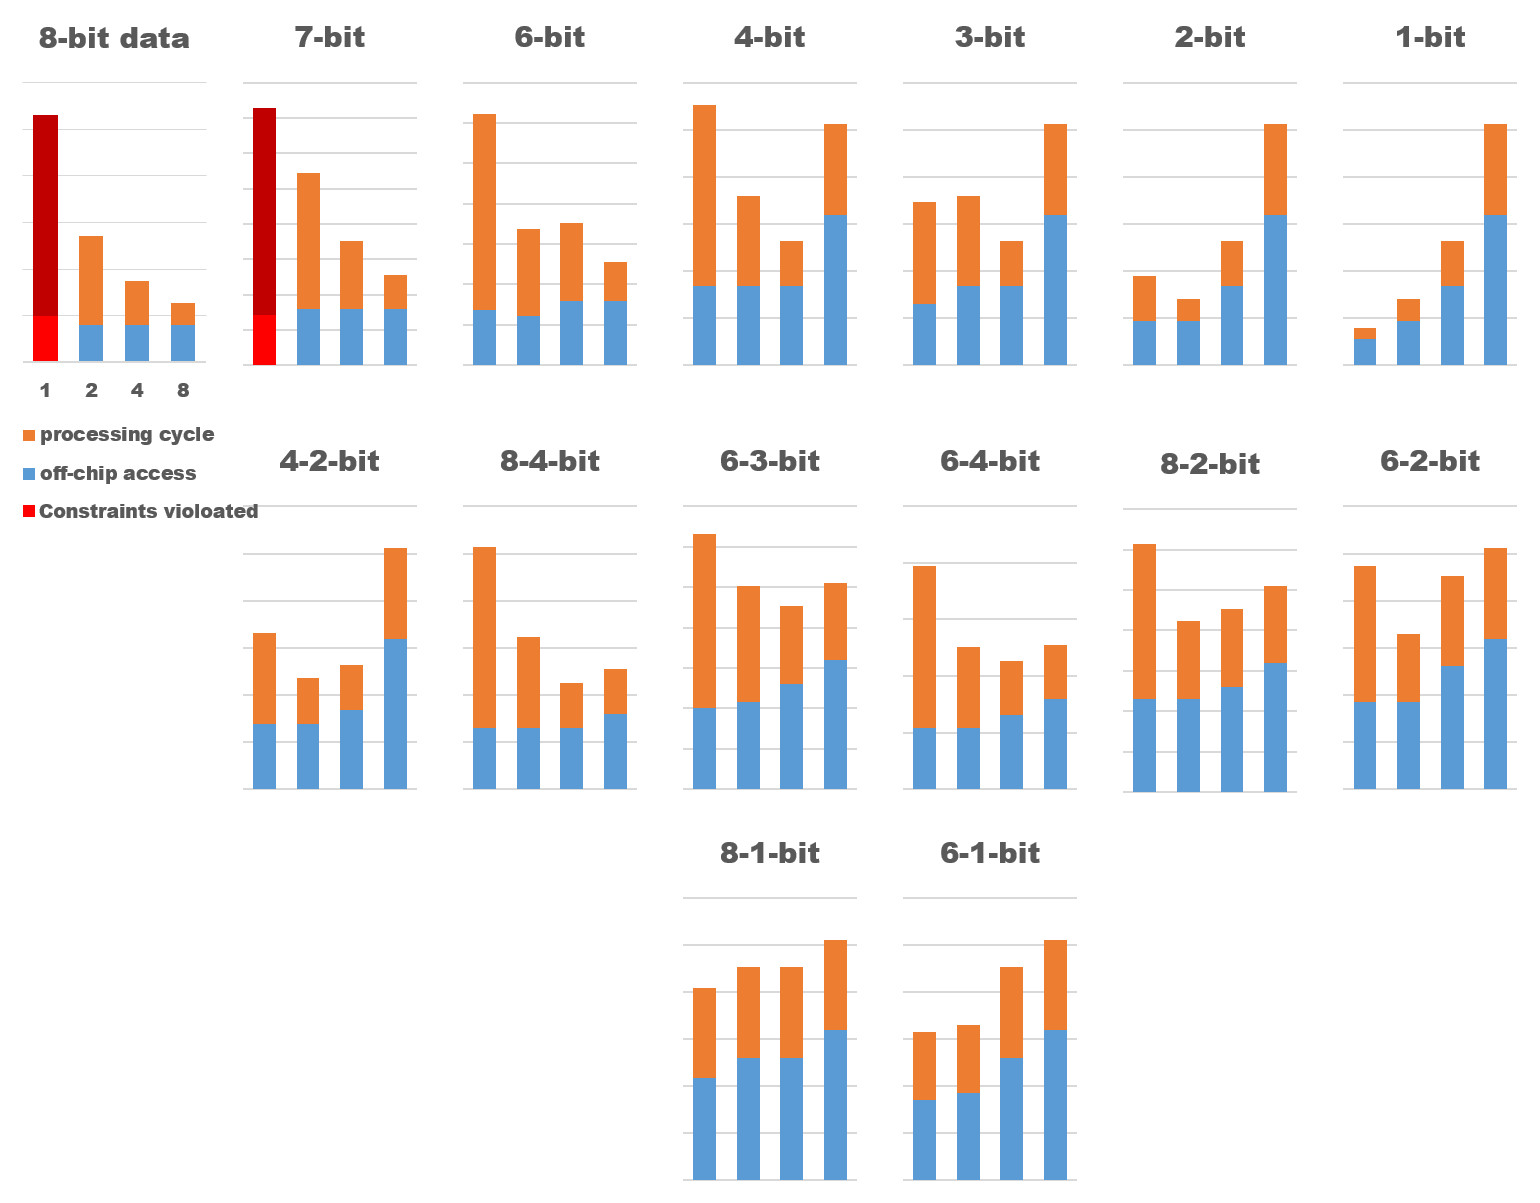
\includegraphics[width=1\linewidth]{inc/5_results/figure/bit_conf.png}
    \caption{Various data bit-length to arithmetic bit-length off-chip access and processing time scaling.}
    \label{fig:bit_conf}
\end{figure}



\chapter{Conclusion}
\label{ch:conclusion}
An architecture capable of performing 1,2,4,8-bit multiplication and add operation on CNN is presented. We set out with the feasibility of linear quantization scheme on CNN, the power consumption bottleneck for deploying CNN on mobile devices, to developing a promising training scheme for linear quantization threshold choosing and achieve $54\%$ accuracy on a 4-bit AlexNet model on ImagenNet dataset, and finally design and implement a precision re-configurable hardware accelerator dedicated to low arithmetic precision CNN networks. The implementation uses 180KB on-chip memory and 1340K logic gates, comparable to existing designs. We synthesized and evaluated the system down to gate-level. The design uses a dataflow suitable for convolution layers with high data reuse rate, couple with a subword accumulation style operation so that the data shape fits onto the on-chip memory properly. We believe this work can benefit low-power mobile deep neural network deployment in practical use.
\iffalse
\textcolor{purple}{Summarise (one or two sentences each) where you set out and what path you went. From that, you should proceed to making clear what kind of advances your results enable. These can be both on the technical (chip design) or on the application level.}
\fi
%syntax references
%\chapter{Syntax/test}

\section{Figure}
\label{sec:figure}
We are from Media IC \& System Lab, as shown in~\figref{misl}.\footnote{All the images in the dissertation are used under Creative Commons license}


\begin{figure}
\begin{center}
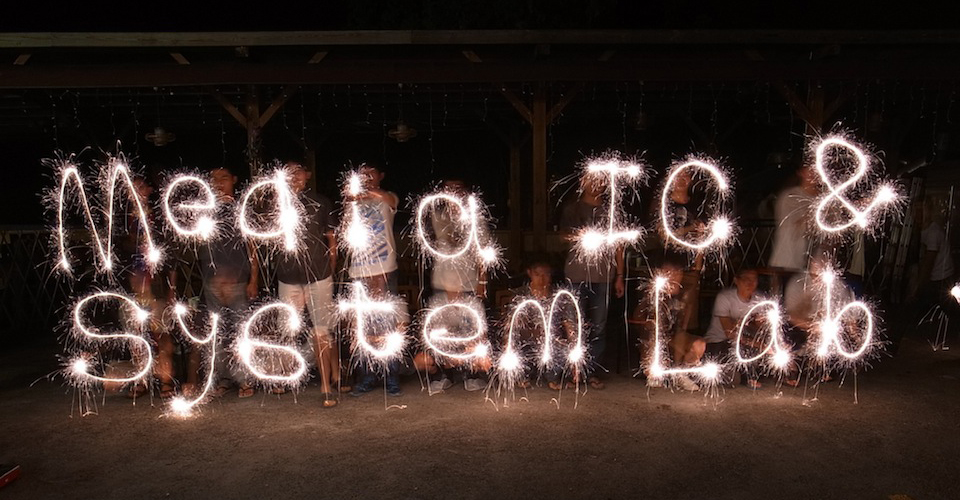
\includegraphics[width=0.8\linewidth]{inc/1_introduction/figure/misl.jpg}
\end{center}
\caption{
We are from Media IC \& System Lab.
}
\label{fig:misl}
\end{figure}


\subsection{Table}
\label{sec:picture}
The related information is shown in~\tabref{lab_information}.

\begin{table}[p]
\vergap{0.8}
\horgap{4.5pt}
\caption{Lab information.}
\vspace{5pt}
\label{tab:lab_information}
\centering
\footnotesize 
\begin{tabular}{cc}
\toprule
Property & Description \\
\midrule
Professor & Shao-Yi Chien \\
Labs & BL421, MD431, MD726 \\
\bottomrule
\end{tabular}
\end{table}


%------------------------------------
% Thesis Body -- end
%------------------------------------

\bibliographystyle{IEEEtran}
\bibliography{thesis}

\end{document}
